\documentclass[openany]{book}

%\usepackage{ctex}
\usepackage{graphicx} 
\usepackage{amsfonts} 
\usepackage{amsthm}    %定理和证明类环境的配置
\usepackage{booktabs}  % 可以使用命令\specialrule 改变表中线的粗细
\usepackage{setspace}
\usepackage{bm}         % 处理数学公式中的黑斜体的宏包
\usepackage{amsmath}    % AMSLaTeX 宏包 用来排出更加漂亮的公式
\usepackage{amssymb}    % AMSLaTeX 宏包 用来排出更加漂亮的公式
\usepackage{color}   %控制颜色的
\usepackage{a0size}     %自由定义字号,在后面“字号设置”中可设置到107pt 为止的大字体
\usepackage{titletoc}  % 设计目录的格式
\usepackage{titlesec}  % 设计标题的格式
\usepackage{fancyhdr}  % 可用来灵活设置页眉和页脚
\usepackage{cite}%产生如(文[2,4-8])的效果
\usepackage{multirow}
\usepackage{float}
\usepackage{geometry}
\usepackage{enumerate}
\usepackage[font=normalsize,labelfont=bf,textfont=bf]{caption}  % 图标的标题字体和自号

\usepackage{polyglossia} %注意,在需要输入英语时使用命令\textenglish{}
\setmainlanguage{russian}
\setotherlanguage{english}
\usepackage{fontspec}
\setmainfont[Ligatures=TeX]{Times New Roman}
\setsansfont{Arial}
\righthyphenmin=2


\DeclareCaptionLabelSeparator{twospace}{\ ~}  % 将图表标题中的冒号改成空格
\captionsetup{labelsep=twospace}

\theoremstyle{definition}
\newtheorem{definition}{Определение}[section]
\newtheorem{remark}{Замечание}[section]
\newtheorem{example}{Пример}[section]
\newtheorem{corollary}{Следствие}[section]
\newtheorem{proposition}{Предложение}[section]
\newtheorem{lemma}{Лемма}[section]
\newtheorem{assumption}{Предположение}[section]
\newtheorem{solution}{Решение}[section]
\newtheorem{property}{Свойства}[section]
\newtheorem{theorem}{Теорема}[section]

\graphicspath{{pics/}} %图片目录
\textwidth 159mm %设置版面宽度
\textheight 246mm %设置版面高度
\topmargin -5mm %设置页面顶端空白的高度
\oddsidemargin 5mm % 设置奇数页的边距
\evensidemargin 5mm  %设置偶数页的边距, 单面时不起作用
\renewcommand\baselinestretch{1.5} %将文本的行间距设为基础行间距的1.5 倍
\renewcommand\arraystretch{0.8} %将数组中的行间距设为基础行间距的2倍
\newcommand{\upcite}[1]{\textsuperscript{\textsuperscript{\cite{#1}}}}  % 将引用的参考文献标号显示为上标
\setlength{\parskip}{3pt plus1pt minus1pt}  % 段落之间的竖直距离

\pagestyle{fancy}          %设置页眉格式
\fancyhead{} %初始化页眉
\fancyhead[CO,CE]{\rightmark}

\geometry{left=2.3cm,right=2.3cm,top=2.8cm,bottom=2.3cm}

\begin{document}



%===================== 重定义字体、字号命令 =============================%
%\newcommand{\song}{\songti}    % 宋体   (Windows 自带simsun.ttf)
%\newcommand{\fs}{\fs}        % 仿宋体 (Windows 自带simfs.ttf)
%\newcommand{\kai}{\kaishu}      % 楷体   (Windows 自带simkai.ttf)
%\newcommand{\hei}{\heiti}      % 黑体   (Windows 自带simhei.ttf)
%\newcommand{\li}{\lishu}        % 隶书   (Windows 自带simli.ttf)
%\newcommand{\you}{\youyuan}      % 幼圆   (Windows 自带simyou.ttf)
\newcommand{\chuhao}{\fontsize{42pt}{\baselineskip}\selectfont}     % 字号设置
\newcommand{\xiaochuhao}{\fontsize{36pt}{\baselineskip}\selectfont} % 字号设置
\newcommand{\yihao}{\fontsize{28pt}{\baselineskip}\selectfont}      % 字号设置
\newcommand{\erhao}{\fontsize{21pt}{\baselineskip}\selectfont}      % 字号设置
\newcommand{\xiaoerhao}{\fontsize{18pt}{\baselineskip}\selectfont}  % 字号设置
\newcommand{\sanhao}{\fontsize{15.75pt}{\baselineskip}\selectfont}  % 字号设置
\newcommand{\xiaosanhao}{\fontsize{14.75pt}{\baselineskip}\selectfont}  % 字号设置
\newcommand{\sihao}{\fontsize{14pt}{\baselineskip}\selectfont}      % 字号设置
\newcommand{\xiaosihao}{\fontsize{12pt}{14pt}\selectfont}  % 字号设置
\newcommand{\wuhao}{\fontsize{10.5pt}{12.6pt}\selectfont}    % 字号设置
\newcommand{\xiaowuhao}{\fontsize{9pt}{11pt}{\baselineskip}\selectfont}   % 字号设置
\newcommand{\liuhao}{\fontsize{7.875pt}{\baselineskip}\selectfont}  % 字号设置
\newcommand{\qihao}{\fontsize{5.25pt}{\baselineskip}\selectfont}    % 字号设置




\def \proof{\indent{Доказательство\ \ } \ignorespaces}
\def \endproof{\vbox{\hrule height0.6pt\hbox{\vrule height1.3ex width0.6pt\hskip0.8ex\vrule width0.6pt}
               \hrule height0.6pt}\vskip 3mm}

\def\solution{\indent{Решение\ \ } \ignorespaces}
\def\endsolution{\vbox{\hrule height0.6pt\hbox{\vrule height1.3ex width0.6pt\hskip0.8ex\vrule width0.6pt}
               \hrule height0.6pt}\vskip 3mm}

\catcode`@=11


% Change definition of \thebibliography environment to use smaller font.
\renewenvironment{thebibliography}[1]
     {\def\chaptername{}\chapter{Список литературы}
     %\thispagestyle{headings}  %使参考文献列表的起始页显示页眉                            !!!
      \list{\@biblabel{\@arabic\c@enumiv}}%
           {\settowidth\labelwidth{\@biblabel{#1}}%
            \leftmargin\labelwidth
            \advance\leftmargin\labelsep
            \@openbib@code
            \usecounter{enumiv}%
            \let\p@enumiv\@empty
            \renewcommand\theenumiv{\@arabic\c@enumiv}}%
      \small%                                               !!!
      \sloppy
      \clubpenalty4000
      \@clubpenalty \clubpenalty
      \widowpenalty4000%
      \sfcode`\.\@m}
     {\def\@noitemerr
       {\@latex@warning{Empty `thebibliography' environment}}%
      \endlist}



%%%%%%%%%%%%%%%%%%%%%%%%%%% 开始章的定义%%%%%%%%%%%%%%%%%%%%%%%%%%%%%%
% Define chapter
\renewcommand\chaptername{Глава\,\thechapter}
\def\@chapter[#1]#2{\ifnum \c@secnumdepth >\m@ne
                           %\pagestyle{empty}%                       !!!
                       \if@mainmatter
                           \pagestyle{headings}%                       !!!
                           \refstepcounter{chapter}%
                          \protected@xdef\@currentlabel{\chaptername}%  !!!
                          \typeout{\erhao \@chapapp \space \thechapter.}%
                          \addcontentsline{toc}{chapter}{\protect\numberline
                          {\xiaosihao\chaptername} {\xiaosihao #1}}%  !!!
                       \else
                          \addcontentsline{toc}{chapter}{\xiaosihao #1}%
                       \fi
                    \else
                       \addcontentsline{toc}{chapter}{\xiaosihao #1}%
                    \fi
                    \chaptermark{#1}%
                    \addtocontents{lof}{\protect\addvspace{10\p@}}%
                  \addtocontents{lot}{\protect\addvspace{10\p@}}%
                    \if@twocolumn
                       \@topnewpage[\@makechapterhead{#2}]%
                    \else
                       \@makechapterhead{#2}%
                       \@afterheading
                    \fi
                    }
\def\@chapapp{Chapter}%                   !!!
\def\chapterformat{\xiaoerhao\bfseries\centering}%      |||
\def\@makechapterhead#1{%

                \if@mainmatter
                          \renewcommand\leftmark{\wuhao \chaptername\ \ \ #1}
                       \else
                          \renewcommand\leftmark{\wuhao #1}%
                       \fi
                         \vspace*{-\headsep}\vspace*{-\headheight}\vspace*{15\p@}%      !!!
                         {\chapterformat%                       !!!
                         \ifnum \c@secnumdepth >\m@ne%                                !!!
                             \if@mainmatter%                                            !!!
                                \chaptername \quad #1 \par\nobreak%      !!!
                             \else%                                                     !!!
                                #1 \par\nobreak%                         !!!
                             \fi%                                                       !!!
                         \fi%                                                         !!!
                         \vskip 15\p@%                                                !!!
                         }
                        }
\def\@makeschapterhead#1{%
                            \vspace*{-\headsep}\vspace*{-\headheight}\vspace*{15\p@}%   !!!
                            {\chapterformat%                        !!!
                             \interlinepenalty\@M%                                     !!!
                             #1\par\nobreak%                                           !!!
                             \vskip 15\p@%                                             !!!
                            }
                         }
%%%%%%%%%%%%%%%%%%%%%%%%%%% 结束章的定义%%%%%%%%%%%%%%%%%%%%%%%%%%%%%%

\renewcommand \thetable
     {\ifnum \c@chapter>\z@ \thechapter -\fi \@arabic\c@table}  % 定义表的编号形式

\renewcommand \thefigure
     {\ifnum \c@chapter>\z@ \thechapter -\fi \@arabic\c@figure}  %定义图的编号形式


\catcode`@=12




\titleformat{\chapter}{\centering\xiaoerhao }{\chaptername}{0.8em}{}
\titlespacing{\chapter}{0pt}{*1}{*1}  % 定义一级标题的格式
\titleformat{\section}{\xiaosanhao}{\hspace*{0.8cm}\thesection }{.8em}{} % 定义二级标题的格式
\titleformat{\subsection}{ \sihao }{ \hspace*{0.8cm}\thesubsection }{.8em}{} % 定义三级标题的格式
\titleformat{\subsubsection}{\large }{ \hspace*{0.8cm}\thesubsubsection }{.8em}{}  % 定义四级标题的格式

%%%%%%%%%%%%%%%%%%%%%%%%%%%%% 封面%%%%%%%%%%%%%%%%%%%%%%%%%%%%%%%%%%%%%%%%%
\vspace*{-1.6cm}

\begin{center}
\begin{figure}[!h]
\hspace*{0mm}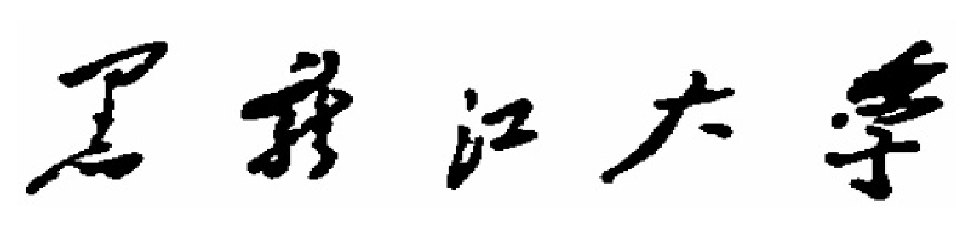
\includegraphics[width=\textwidth]{cover.eps}
%\caption{dblfgb}
  \end{figure}

\vspace*{3mm} \hspace*{0mm}{\yihao Дипломная\hspace{1.8mm} работа}

\end{center}

\vspace{2mm}

{\xiaosanhao
$$
\begin{array}{l}
\hbox{Тема:}\hspace{4.7cm}$\underline{\makebox[10.2cm][l]{\sihao Компактный оператор и их применение}}$\\[5.5mm]
\hbox{Институт:}\hspace{3.7cm}$\underline{\makebox[10.2cm][l]{Китайско-российский Институт}}$\\[5.5mm]
\hbox{Курс:}\hspace{4.8cm}$\underline{\makebox[10.2cm][l]{2019}}$\\[5.5mm]
\hbox{Специальность:}\hspace{2.5cm}$\underline{\makebox[10.2cm][l]{Математика и прикладная математика}}$\\[5.5mm]
\hbox{Фамилия и имя:}\hspace{2.5cm}$\underline{\makebox[10.2cm][l]{Ань Чжаолун}}$\\[5.5mm]
\hbox{Номер студента:}\hspace{2.4cm}$\underline{\makebox[10.2cm][l]{20191236}}$\\[5.5mm]
\hbox{Научный руководитель:}\hspace{8mm}$\underline{\makebox[10.2cm][l]{Ван Шимо}}$
\end{array}
$$
}
\vspace{24mm}

\begin{center}
{\sihao 5\hspace{1.8mm} мая\hspace{1.8mm}2023\hspace{1.8mm} г.} %日期
\end{center}
%%%%%%%%%%%%%%%%%%%%%%%%%%%%%%%%%%%%%%%%%%%%%%%%%%%%%%%%%%%%%%%%%%%%%%%%%%


\pagestyle{empty} %页眉为空

\frontmatter

\chapter{Конспект}
\renewcommand{\thepage}{\Roman{page}} %从现在开始页号为大写罗马体
Тесные операторы обладают многими важными свойствами, такими как конечная размерность, замкну\-тость и непрерывность, и широко используются в математике и физике. 
На практике основная цель тесных операторов - преобразовать задачи бесконечной размерности в задачи конечной размерности, тем самым делая анализ и решение задач более простыми и выполнимыми.
Это делает анализ и решение задачи более простым и выполнимым.

В данной статье дается краткое введение в понятие тесных операторов и рассматриваются примеры применения тесных операторов в математике.
Во-первых, в статье дается определение и свойства плотных операторов и их хорошие арифметические свойства, а также приводятся некоторые основные примеры плотных операторов.
Наконец, в конце статьи приводится краткое описание применения узких операторов в математике.

Переведено с помощью www.DeepL.com/Translator (бесплатная версия)



\vspace{1.5cm}
\begin{center}
    {\bfseries Ключевые слова}

\end{center}





\newpage  %去掉正文前空白页的页眉和页脚
\thispagestyle{empty}


\newpage
\makeatletter
\renewcommand*\l@chapter{\@dottedtocline{0}{0em}{5em}}
\makeatother

\tableofcontents   %自动生成目录表

\mainmatter  %开始正文部分
\chapter{Введение}  %章标题
\pagestyle{fancy}
\renewcommand{\thepage}{\arabic{page}} %从正文开始页号显示为阿拉伯数字

\setcounter{page}{1}  %从正文开始页号重新编号

\section{Значение исследования темы}



\section{Структура работы}



\chapter{Заголовок}    %章标题
\pagestyle{fancy}


\chapter{Компактный оператор}
\pagestyle{fancy}


\section{Заголовок}




\section{Заголовок}


\chapter{Заголовок}
\pagestyle{fancy}
\section{Заголовок}

\section{Заголовок}


\section{Заголовок}


\section{Выводы главы}


\chapter{Заголовок}
\pagestyle{fancy}


\section{Заголовок}






\section{Выводы главы}



\chapter{Заголовок}
\pagestyle{fancy}

\section{Заголовок}



\chapter{Итоги}\label{ch7}
\pagestyle{fancy}

\backmatter

%一次管理,一次使用
%参考文献格式:
% \begin{thebibliography}{编号样本}
%   \bibitem[记号]{引用标志}文献条目1
%   \bibitem[记号]{引用标志}文献条目2
%   ······
% \end{thebibliography}
%其中文献条目包括:作者,题目,出版社,年代,版本,页码等。
%引用时候要可以采用: \cite{引用标志1,引用标志2,···}
\begin{thebibliography}{99}
    \bibitem{book1}\textenglish{William H. Press, Sual A. Teukolsky, William T. Vetterling, Brian P. Flannery, \emph{Numerical Recipes 3rd Edition: The Art of Scientific Computing}
    Cambridge University Press, New York, 2007.}
    \bibitem{latexGuide}\textenglish{Kopka Helmut, W. Daly Patrick,
    \emph{Guide to \text{\LaTeX}}, $4^{th}$ Edition. Available at \texttt{http://www.amazon.com}.}
    \bibitem{latexMath}\textenglish{Graetzer George, \emph{Math Into \text{\LaTeX}},
    BirkhAuser Boston; 3 edition (June 22, 2000).}    
\end{thebibliography}


\chapter{Благодарности}
\pagestyle{fancy}

\end{document}